\documentclass{article}

% Language setting
\usepackage[english]{babel}
\usepackage[utf8]{inputenc}
\usepackage[T1]{fontenc}

% Set page size and margins
\usepackage[letterpaper,top=2cm,bottom=2cm,left=3cm,right=3cm,marginparwidth=1.75cm]{geometry}

% Useful packages
\usepackage{amsmath}
\usepackage{amsthm}
\usepackage{amssymb}
\usepackage{graphicx}
\usepackage{comment}
\usepackage{amsmath}
\usepackage{xcolor}
\usepackage{float}

\usepackage{parskip}
\usepackage[most]{tcolorbox}
\usepackage[colorlinks=true, allcolors=blue]{hyperref}
\usepackage[english]{cleveref}

\definecolor{cremeSepia}{RGB}{245, 242, 235}

% Creation of environments automatically numbered in the preamble
\newtcbtheorem[auto counter]{definicao}{Definition}{
	colback=blue!1,
	colframe=blue!75!white,
	fonttitle=\bfseries
}{def}

\newtcbtheorem[auto counter]{teorema}{Theorem}{
	colback=blue!1,
	colframe=blue!75!white,
	fonttitle=\bfseries
}{teo}

\title{VARIATIONAL FORMULATIONS I: Abstract problems.\\
	Computational}
\author{Victor Matheus da Cunha Santos\\
	NUSP: 13279534}

\begin{document}
	\maketitle
	\pagecolor{cremeSepia}
	
	\section*{Problem}	
	Given the computational domain $\Omega=\left[0, L_x\right] \times\left[0, L_y\right] \subset \mathbb{R}^2, \partial \Omega=$ $\Gamma_{\text {left }} \cup \Gamma_{\text {ad }} \cup \Gamma_{\text {right }}$, source term $f$ and thermal diffusivity $\mu$, find temperature field $u$ satisfying
	
	$$
	\left\{\begin{array}{rlrl}
		-\nabla \cdot(\mu(\mathbf{x}) \nabla u(\mathbf{x})) & =f(\mathbf{x}) & \mathbf{x} \in \Omega \\
		u(\mathbf{x}) & =u_{\ell} & & \mathbf{x} \in \Gamma_{\text {left }} \\
		u(\mathbf{x}) & =u_r & & \mathbf{x} \in \Gamma_{\text {right }} \\
		-\mu(\mathbf{x}) \nabla u(\mathbf{x}) \cdot \check{\mathbf{n}}(\mathbf{x}) & =0 & & \mathbf{x} \in \Gamma_{\text {ad }}
	\end{array}\right.
	$$
	The thermal diffusivity $\mu$ is piecewise constant and defined by
	$$
	\mu(\mathbf{x})=\left\{\begin{array}{lll}
		\mu_B & \text { if } & \mathbf{x} \in \Omega_B=\cup_{i=1}^{n_b} \omega_i, \omega_i=\left\{\mathbf{x} \in \Omega,\left\|\mathbf{x}-\mathbf{x}_c^i\right\|<r_i\right\} \\
		\mu_A & \text { if } & \mathbf{x} \in \Omega_A=\Omega \backslash \Omega_B
	\end{array}\right.
	$$	
	
	
	\section{Exercise 1}
	In the problem there are two types of boundary conditions and each one is applied in different ways; Neumann-type boundary conditions are imposed in the variational formulation of the problem, when we integrate by parts the terms where the solution condition appears strongly, the flux boundary conditions appear naturally, and in this case we can apply the conditions that define the problem. On the other hand, Dirichlet conditions are imposed on the solution search space; in this case, we choose the space of continuous functions of degree 1, that is, piecewise linear functions. Below we write the variational formulation and apply the boundary conditions.
	\subsection*{Variational Formulation}
	
	\noindent \textbf{Vector identity:}
	
	For a vector field $\mathbf{F}$ and a scalar function $v$,
	\begin{equation*}
		\nabla\cdot(v\mathbf{F})
		=
		v\,\nabla\cdot\mathbf{F}
		+
		\mathbf{F}\cdot\nabla v.
	\end{equation*}
	
	\noindent \textbf{Function spaces:}
	
	We define the test function space by
	\begin{equation*}
		V_0
		=
		\left\{
		v\in H^1(\Omega):
		v=0 \text{ on }
		\Gamma_{\mathrm{left}}\cup\Gamma_{\mathrm{right}}
		\right\}.
	\end{equation*}
	
	The solution is sought in the set
	\begin{equation*}
		V_g
		=
		\left\{
		u\in H^1(\Omega):
		u=u_\ell \text{ on }\Gamma_{\mathrm{left}},
		\quad
		u=u_r \text{ on }\Gamma_{\mathrm{right}}
		\right\},
	\end{equation*}
	where the boundary conditions are understood in the trace sense.
	
	\noindent \textbf{Integrated equation:}
	
	Multiplying the Poisson equation by a test function $v\in V_0$
	and integrating over the domain, we obtain
	\begin{equation}
		-\int_\Omega
		\nabla\cdot(\mu\nabla u)\,v\,dx
		=
		\int_\Omega fv\,dx.
		\label{eq:poisson-integrada}
	\end{equation}
	
	Using the vector identity with $\mathbf{F}=\mu\nabla u$,
	\begin{equation*}
		-v\,\nabla\cdot(\mu\nabla u)
		=
		-\nabla\cdot(v\mu\nabla u)
		+
		\mu\nabla u\cdot\nabla v.
	\end{equation*}
	
	Therefore,
	\begin{equation*}
		-\int_\Omega
		\nabla\cdot(v\mu\nabla u)\,dx
		+
		\int_\Omega
		\mu\nabla u\cdot\nabla v\,dx
		=
		\int_\Omega fv\,dx.
	\end{equation*}
	
	Applying Gauss's Theorem to the divergence term,
	\begin{equation*}
		\int_\Omega
		\nabla\cdot(v\mu\nabla u)\,dx
		=
		\int_{\partial\Omega}
		\mu\nabla u\cdot\mathbf{n}\,v\,ds,
	\end{equation*}
	where $\mathbf{n}$ is the unit outward normal to the domain.
	
	Thus, integration by parts gives
	\begin{equation*}
		\int_\Omega
		\mu\nabla u\cdot\nabla v\,dx
		-
		\int_{\partial\Omega}
		\mu\nabla u\cdot\mathbf{n}\,v\,ds
		=
		\int_\Omega fv\,dx.
	\end{equation*}
	
	Since the boundary is divided into
	\begin{equation*}
		\partial\Omega
		=
		\Gamma_{\mathrm{left}}
		\cup
		\Gamma_{\mathrm{right}}
		\cup
		\Gamma_{\mathrm{ad}},
	\end{equation*}
	we obtain
	\begin{equation*}
		\begin{aligned}
			\int_\Omega \mu\nabla u\cdot\nabla v\,dx
			&-
			\int_{\Gamma_{\mathrm{left}}}
			\mu\nabla u\cdot\mathbf{n}\,v\,ds
			-
			\int_{\Gamma_{\mathrm{right}}}
			\mu\nabla u\cdot\mathbf{n}\,v\,ds
			\\
			&-
			\int_{\Gamma_{\mathrm{ad}}}
			\mu\nabla u\cdot\mathbf{n}\,v\,ds
			=
			\int_\Omega fv\,dx.
		\end{aligned}
	\end{equation*}
	
	\noindent \textbf{Application of boundary conditions:}
	
	On the Dirichlet boundaries, the boundary terms vanish because
	\begin{equation*}
		v=0
		\quad\text{on}\quad
		\Gamma_{\mathrm{left}}\cup\Gamma_{\mathrm{right}}.
	\end{equation*}
	
	On the adiabatic walls, the boundary term vanishes due to the
	homogeneous Neumann condition:
	\begin{equation*}
		-\mu\nabla u\cdot\mathbf{n}=0
		\quad\text{on}\quad
		\Gamma_{\mathrm{ad}}.
	\end{equation*}
	
	Consequently, the variational formulation consists of finding
	$u\in V_g$ such that
	\begin{equation}
		\underbrace{
			\int_\Omega \mu\nabla u\cdot\nabla v\,dx
		}_{a(u,v)}
		=
		\underbrace{
			\int_\Omega fv\,dx
		}_{\ell(v)}
		\qquad\forall v\in V_0.
		\label{eq:poisson-variacional}
	\end{equation}
	
	The Dirichlet conditions are incorporated into the search set
	$V_g$. The adiabatic condition is naturally incorporated into the
	variational formulation by the cancellation of the flux term on the upper
	and lower walls.
	
	For discontinuous $\mu$ at the inclusion interfaces, integration
	by parts can be performed in each region. In the derivation from a
	sufficiently piecewise-regular solution, the contributions
	from the interfaces cancel due to the continuity of the normal flux and
	the use of test functions from $H^1(\Omega)$.
	
	
	
	\vspace{1cm}
	\noindent \textbf{Discrete forms:}
	\begin{align*}
		a &= \text{inner}(\text{mu} \ast \text{grad}(u), \text{grad}(v)) \, dx \\
		l &= f \, v \, dx
	\end{align*}
	
	\subsection*{Zero Flux}
	The zero flux is imposed on the top and bottom walls; it is a Neumann-type condition that indicates the absence of normal heat flux. In this case it is applied on the walls
	\[
	\mu(x) \nabla u(x) \cdot \hat{n} = 0
	\]
	
	\noindent \textbf{}
	\begin{figure}[H]
		\centering
		\caption[Visual scheme of elements and faces]{}
		\label{fig:boundaries}
		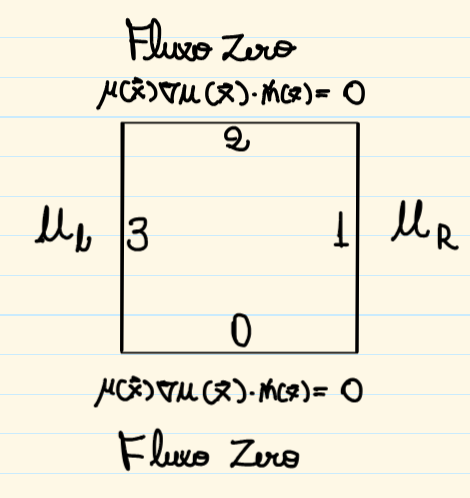
\includegraphics[width=0.4\linewidth]{boundaries}
	\end{figure}
	
	
	\noindent \textbf{Where do $u_l$ and $u_r$ enter?}
	
	\noindent A tag is created for each wall.
	\[
	\text{bcs} = \{ (V_h, \text{u\_left}, 3), (V_h, \text{u\_right}, 1) \}
	\]
	
	\section{Exercise 2}
	
	
	\begin{figure}[H]
		\centering
		\caption{}
		\label{fig:meshsurface}
		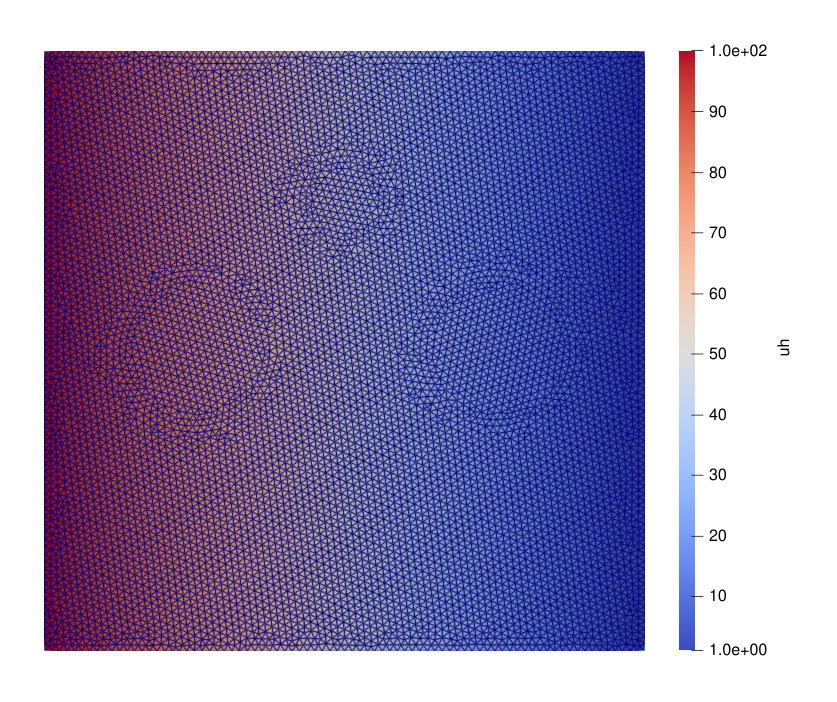
\includegraphics[width=0.4\linewidth]{mesh_surface}
	\end{figure}
	
	
	\section{Exercise 3 - 4}
	\subsection{Norms}
	\begin{equation}
		\|u - u_{h}\|_{H^{1}} = \left( \int_{\Omega} (u - u_{h})^{2} + \| \nabla(u - u_{h}) \|^{2} dx  \right) ^{1/2}
	\end{equation}
	
	\begin{equation}
		\|u - u_{h}\|_{L^{2}} = \left( \int_{\Omega} (u - u_{h})^{2} dx  \right) ^{1/2}
	\end{equation}
	\subsection{Comparison between situations}
	With the situation where we have zero source and non-homogeneous Dirichlet conditions ($u_l = 100, ~ u_r = 1$ and $f = 0$), for the following analytical solution:
	
	\begin{equation}
		u_e(\mathbf{x}) = u_{\ell} - \frac{u_{\ell} - u_r}{L_x} x
	\end{equation}
	
	\begin{figure}[H]
		\centering
		\caption{}
		\label{fig:perfiltransversaluh}
		\includegraphics[width=0.4\linewidth]{figures/perfil_transversal_uh_uexata}
	\end{figure}
	
	\begin{table}[H]
		\centering
		\caption{Approximation errors}
		\label{tab:erros}
		\begin{tabular}{lc}
			\hline
			\textbf{Error} & \textbf{Value} \\
			\hline
			$L^2$ error & $1.114 \times 10^{-12}$ \\
			$H^1$ error & $4.267 \times 10^{-12}$ \\
			\hline
		\end{tabular}
	\end{table}
	With the situation where we have non-zero source and homogeneous Dirichlet conditions ($u_l = 0, ~ u_r = 0$ and $f = 100$), for the following analytical solution:
	
	\begin{equation}
		u_e(\mathbf{x}) = 50*x(L_x - x).
	\end{equation}
	
	\begin{figure}[H]
		\centering
		\caption{}
		\label{fig:perfiltransversal_f100}
		\includegraphics[width=0.4\linewidth]{figures/perfil_transversal_uh_uexata_f100}
	\end{figure}
	
	\begin{table}[htbp]
		\centering
		\caption{Error norms since analytical solution is available ($\mu_A=\mu_B$ and $f=0$)}
		\label{tab:error-norms}
		\begin{tabular}{lc}
			\hline
			\textbf{Error} & \textbf{Value} \\
			\hline
			$L^2$ error & $0.008521501512041887$ \\
			$H^1$ error & $1.2456604608567208$ \\
			\hline
		\end{tabular}
	\end{table}
	
	When we study the error between \(u\) and \(u_h\), when \(u\) is a linear function, it is verified that the function space to which \(u_h\) belongs (CG1), that is, continuous piecewise linear functions of degree one, represents exactly the characteristics of \(u\). Furthermore, \(u'\) is constant and \(u_h'\) is also constant; in this situation the choice of space is appropriate. On the other hand, when \(u\) is a quadratic function, CG1 becomes a less adequate function space, since \(u'\) is now linear while \(u_h'\) is constant; comparing graphically,
	
	
	\begin{figure}[H]
		\centering
		\caption{}
		\label{fig:erro_interpret}
		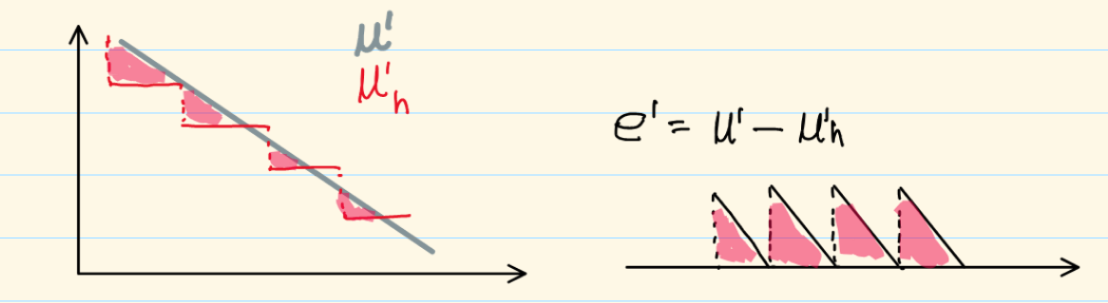
\includegraphics[width=0.6\linewidth]{figures/erros_interpret}
	\end{figure}
	
	Besides what happens with \(u'\) and \(u_h'\), in the case where \(u\) is quadratic and \(u_h\) is in CG1,
	
	\begin{figure}[H]
		\centering
		\caption{}
		\label{fig:erro_quadratica}
		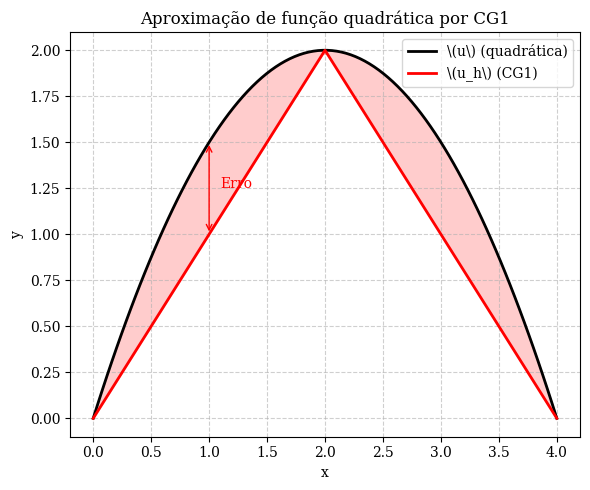
\includegraphics[width=0.4\linewidth]{figures/cg1_quadratica}
	\end{figure}
	
	
	In fact, the \(H^1(\Omega)\) norm is more suitable for seeing what happens with \(u'\) and \(u_h'\).
	
	
	\begin{comment}
		
		
		\begin{figure}[H]
			\centering
			\begin{minipage}{0.48\linewidth}
				\centering
				\caption{}
				\label{fig:ueuh}
				\includegraphics[width=\linewidth]{ue_uh}
			\end{minipage}
			\hfill
			\begin{minipage}{0.48\linewidth}
				\centering
				\caption{}
				\label{fig:ueuh_f100}
				\includegraphics[width=\linewidth]{ue_uh_f100}
			\end{minipage}
		\end{figure}
	\end{comment}
	
	\section{Exercise 7}
	In the first situation, zero source and non-homogeneous Dirichlet conditions ($u_l = 100,  u_r = 1$ and $f = 0$), we compute the effective thermal diffusivity,
	
	\begin{equation}
		\mu_{eff} = \frac{|Q| / L_{y}}{|u_{l} - u_{r}|/L_{x}}
	\end{equation}
	
	\begin{table}[htbp]
		\centering
		\caption{Simulation results}
		\label{tab:resultados_nonhomogen}
		\begin{tabular}{lc}
			\hline
			\textbf{Quantity} & \textbf{Value} \\
			\hline
			$Q_{in}$ & $99.00$ \\
			$Q_{out}$ & $98.99$ \\
			Power & $0.0$ \\
			Balance residual & $-3.282 \times 10^{-12}$ \\
			$\mu_{eff}$ & $0.999$ \\
			\hline
		\end{tabular}
	\end{table}
	It is verified from \cref{tab:resultados_nonhomogen} that, with the result that when ($\mu_{A} = \mu_{B} = 1$) the \(\mu_{eff}\) recovers this value; physically we can say that the domain is a single material.
	The coefficient \(\mu\) relates the temperature variation ($\nabla u$) to the heat flux $\mathbf q$:
	\begin{equation*}
		\mathbf q=-\mu\nabla u.
	\end{equation*}
	This means that, for the same temperature gradient, a material with higher \(\mu\) allows a greater heat flux. The product of $\mu$ with ($\nabla u$) represents a scalar multiplying a vector field, which modifies the magnitude of the resulting vectors; in this case the heat flux increases or decreases depending on $\mu$. The negative sign indicates that heat flows from the hotter region to the colder one.
	For a homogeneous material, the temperature varies linearly, and the magnitude of the gradient is
	\begin{equation*}
		|\nabla u|=\frac{|u_\ell-u_r|}{L_x}.
	\end{equation*}
	Thus, the flux per unit area is
	\begin{equation*}
		|q_x|=\mu\frac{|u_\ell-u_r|}{L_x}.
	\end{equation*}
	Since \(Q\) is the flux integrated over the lateral side of length \(L_y\), we have \(|Q|/L_y=|q_x|\), in the two-dimensional interpretation per unit thickness. Isolating the coefficient:
	\begin{equation*}
		\mu_{\mathrm{eff}}
		\frac{|Q|/L_y}{|u_\ell-u_r|/L_x}.
	\end{equation*}
	
	
	\section{Exercise 8}
	\begin{table}[H]
		\centering
		\caption{Simulation results}
		\label{tab:resultados_exe8}
		\begin{tabular}{lc}
			\hline
			\textbf{Quantity} & \textbf{Value} \\
			\hline
			$Q_{in}$ & $-197.89$ \\
			$Q_{out}$ & $197.81$ \\
			Power & $400.00$ \\
			$ - Q_{in} + Q_{out}$ & $395.70$ \\
			Balance residual & $-4.2900$ \\
			\hline
		\end{tabular}
	\end{table}
	
	
	\section{Exercise 9}
	With the following parameters, \(\mu_A=5\), \(\mu_B=500\), \(f=100\), \(u_\ell=u_r=0\)
	\begin{figure}[H]
		\centering
		\caption{}
		\label{fig:exe9}
		\includegraphics[width=0.4\linewidth]{figures/exe_9}
	\end{figure}
	
	\section{Exercise 10}
	\begin{equation*}
		E_i(h)
		\left|
		\overline T_i^h-\overline T_i^{\mathrm{ref}}
		\right|.
	\end{equation*}
	
	
	\begin{figure}[H]
		\centering
		\caption{}
		\label{fig:exe10}
		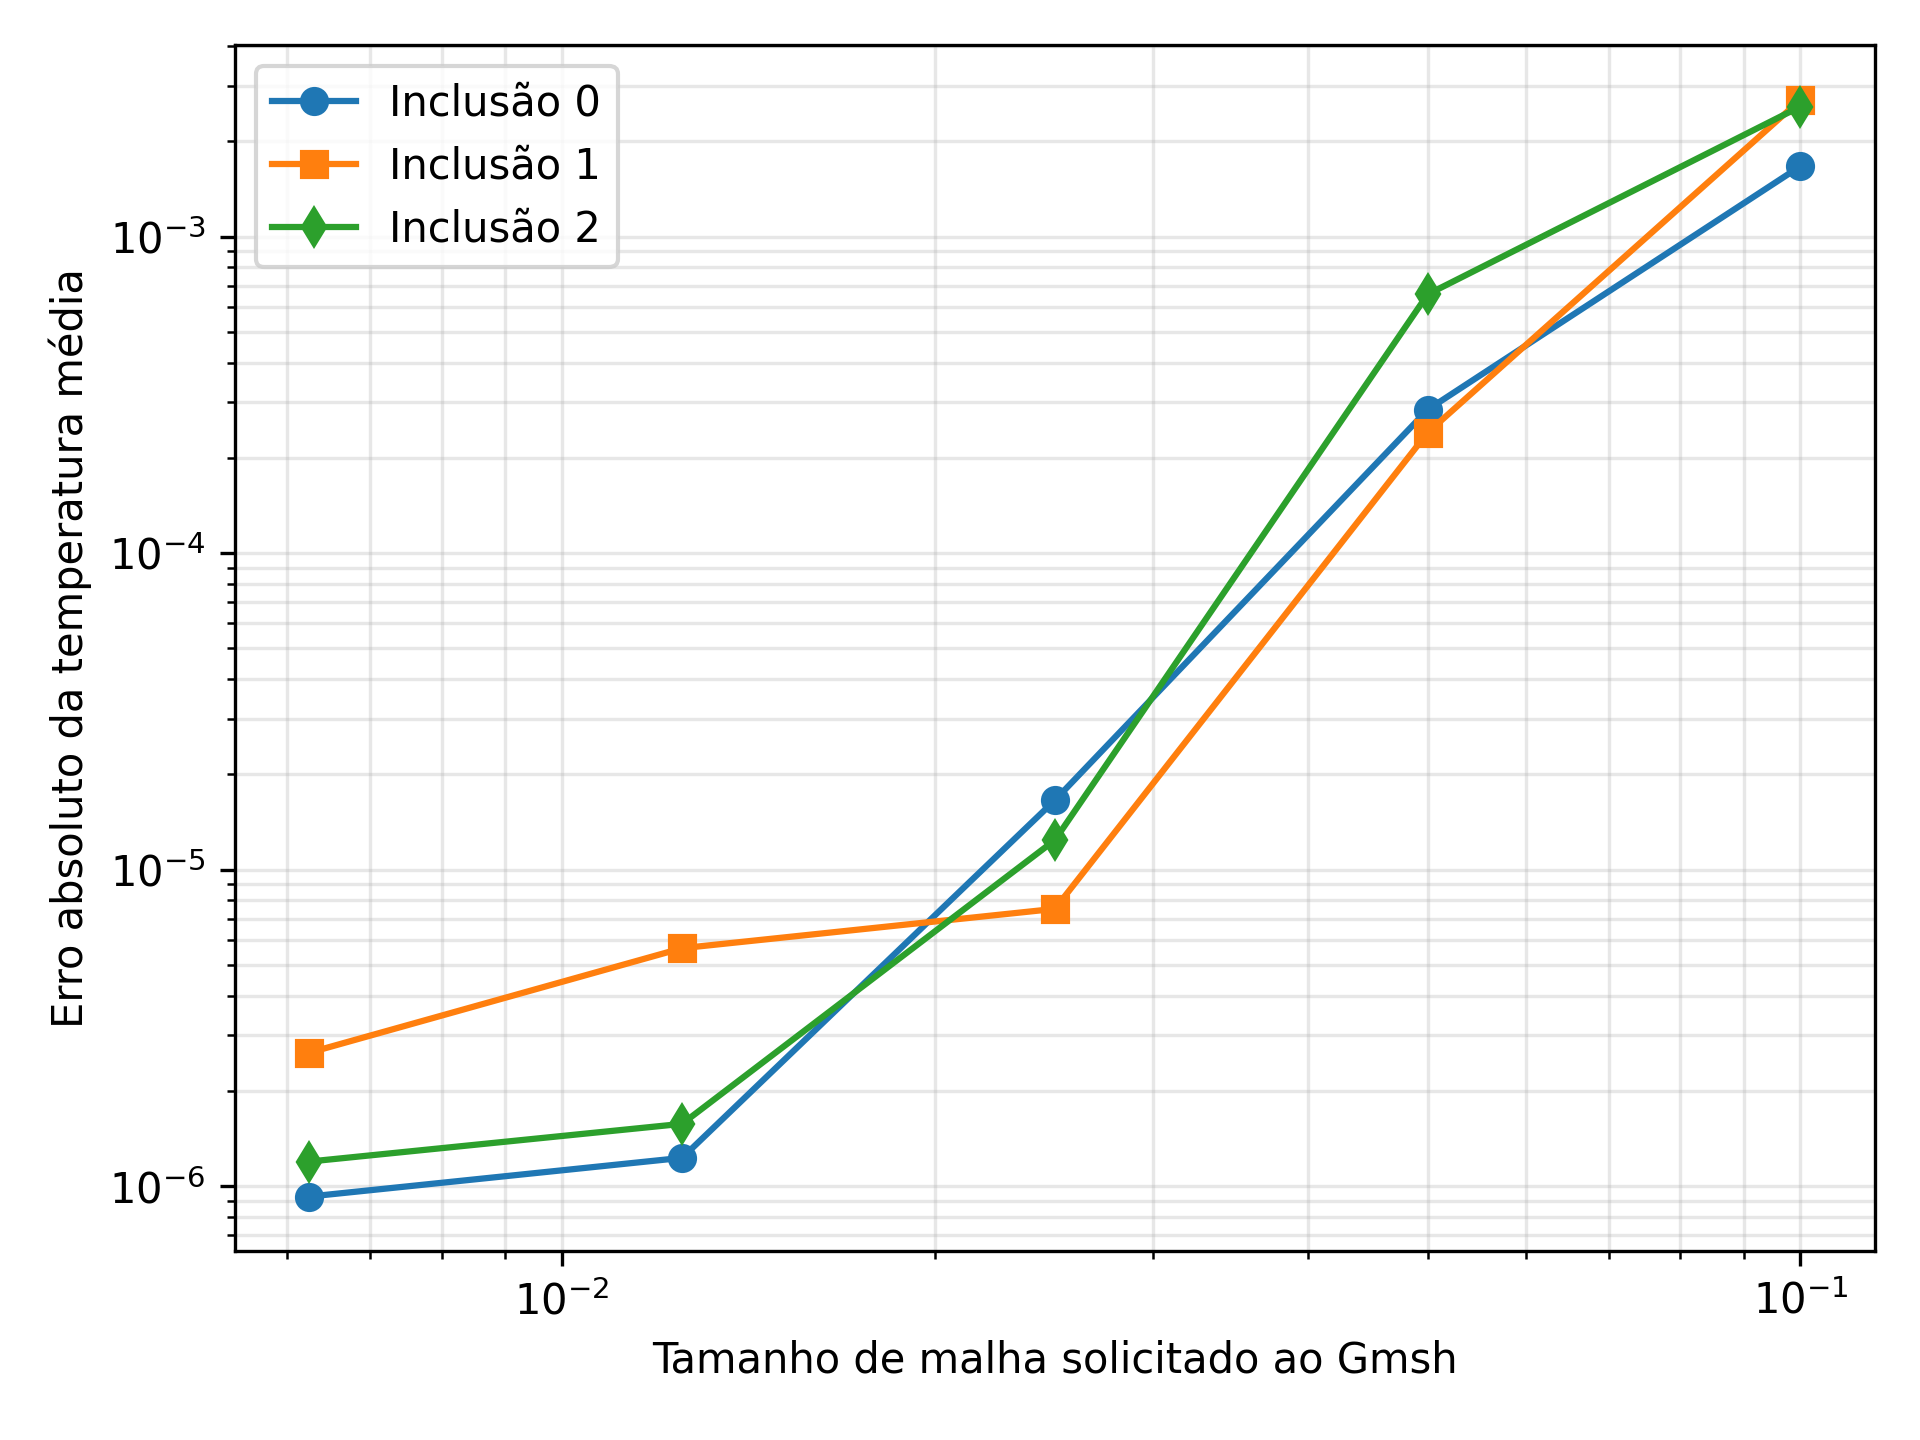
\includegraphics[width=0.4\linewidth]{figures/converg}
	\end{figure}
	\begin{table}[H]
		\centering
		\caption{Average temperatures in the inclusions and absolute errors relative to the reference mesh. The ``Elements'' column shows the total count
			reported by the mesh generator.}
		\label{tab:medias-inclusoes}
		\begin{tabular}{ccccccccc}
			\hline
			$h$ & Nodes & Elements & $T_0$ & $T_1$ & $T_2$ & $E_0$ & $E_1$ & $E_2$ \\
			\hline
			0.10000 & 565     & 1.177   & 6.098348 & 8.115329 & 6.097441 & $1.67\times10^{-3}$ & $2.70\times10^{-3}$ & $2.58\times10^{-3}$ \\
			0.05000 & 2.054   & 4.196   & 6.099733 & 8.117793 & 6.099360 & $2.84\times10^{-4}$ & $2.40\times10^{-4}$ & $6.57\times10^{-4}$ \\
			0.02500 & 7.738   & 15.645  & 6.100000 & 8.118040 & 6.100029 & $1.66\times10^{-5}$ & $7.52\times10^{-6}$ & $1.24\times10^{-5}$ \\
			0.01250 & 30.302  & 60.937  & 6.100018 & 8.118039 & 6.100018 & $1.23\times10^{-6}$ & $5.65\times10^{-6}$ & $1.58\times10^{-6}$ \\
			0.00625 & 119.756 & 240.172 & 6.100018 & 8.118036 & 6.100018 & $9.28\times10^{-7}$ & $2.64\times10^{-6}$ & $1.20\times10^{-6}$ \\
			0.00313 & 475.831 & 952.975 & 6.100017 & 8.118033 & 6.100017 & --- & --- & --- \\
			\hline
		\end{tabular}
	\end{table}
	We can verify that the errors of the three average temperatures decrease with refinement, even though the reduction rates vary between meshes. The averages close to \(6{,}100017\), \(8{,}118033\) and \(6{,}100017\) indicate stabilization of these values relative to the reference used, which was $h_{\mathrm{ref}}=0.003125$ and 475{,}831 nodes.
\end{document}